\documentclass{article}
\usepackage[preprint]{acl}

\usepackage[utf8]{inputenc}
\usepackage[T1]{fontenc}
\usepackage{times}
\usepackage{inconsolata}
\usepackage{booktabs}
\usepackage{amsmath}
\usepackage{amssymb}
\usepackage{amsfonts}
\usepackage{microtype}
\usepackage{graphicx}
\usepackage{subcaption}
\usepackage{tabularx}
\usepackage{tikz}
\usetikzlibrary{arrows.meta}

\graphicspath{{figures/}}




\title{Beyond Endpoint Confidence:\\
Characterizing Uncertainty Across Reasoning Trajectories}

\author{Jerry Chen \quad Gaurav Kamath \quad Siva Reddy \\
  School of Computer Science, McGill University \\
  Mila -- Quebec AI Institute \quad $\cdot$ \quad COMP 400 Research Project Report \\
  \texttt{jerry.chen@mail.mcgill.ca}}

\begin{document}

\maketitle

\begin{abstract}
Reasoning language models generate extended trajectories before producing a final answer, creating an opportunity to study reliability throughout reasoning rather than only at the endpoint. We examine reasoning-token entropy, answer-choice entropy, and verbalized confidence across 5{,}000 stochastic reasoning trajectories generated by SmolLM3-3B on 500 MMLU questions. We find that these signals evolve differently and become informative at different stages of reasoning. Reasoning-token entropy provides its strongest discrimination of final-answer correctness relatively early, while the model's probability distribution over candidate answers becomes increasingly concentrated later in reasoning. This increasing certainty occurs for responses that ultimately yield both correct and incorrect answers, while verbalized confidence remains consistently high despite substantial changes in predictive uncertainty. We also find that the separation between correct and incorrect outcomes for both entropy measures becomes much smaller when comparisons are restricted to the same questions. Together, these findings show that reliability signals capture different aspects of model behaviour, and that their interpretation depends both on when they are measured and on whether correctness is evaluated across or within questions.
\end{abstract}



\section{Introduction}
\label{sec:introduction}

Large language models can approach complex problems by generating a sequence of intermediate steps before committing to a final answer. Chain-of-thought prompting demonstrated that eliciting such steps can improve performance on arithmetic, commonsense, and symbolic reasoning tasks \cite{wei2022chain}. Building on this idea, recent language models are trained to generate extended reasoning trajectories that devote more inference-time computation to complex problems, which can improve performance when used effectively \cite{snell2025scaling,guo2025deepseek}; in this work, we refer to such models as \emph{reasoning language models}. Importantly, the intermediate steps generated by these models form an observable reasoning trajectory that can be studied alongside the answer it ultimately produces.

Despite these gains, extended reasoning does not guarantee a reliable answer. A model can produce a detailed and coherent reasoning trajectory while still reaching an incorrect conclusion \cite{turpin2023unfaithful}. Moreover, strong average performance across a benchmark does not guarantee the accuracy of any individual response. This response-level reliability problem is especially consequential in high-stakes domains such as medicine and law, where incorrect outputs can lead to harmful clinical guidance or inaccurate legal advice \cite{longwell2024medical,dahl2024legal}. These risks create a need for signals that can assess the reliability of individual outputs.

Uncertainty quantification offers one approach to assessing the reliability of individual language-model outputs \cite{geng2024survey}. Broadly, uncertainty quantification studies methods for characterizing how uncertain a model is about its responses, with the aim of assessing how much those responses should be trusted. Prior work has proposed a range of signals derived from model predictions, repeated generations, and self-reported measures of confidence to characterize uncertainty at the level of individual responses \cite{kuhn2023semantic,tian2023calibration,kadavath2022know}.

Assessing uncertainty only at the end of a problem-solving process can obscure how certainty developed along the way. Two people may arrive at the same answer and report equally high confidence, even if one maintained the same answer throughout while the other reconsidered competing alternatives before becoming certain. Reasoning models, however, offer new possibilities for examining this process because their generated trajectories can be studied at multiple stages before the final answer is produced. Recent work has shown that uncertainty can change systematically throughout chain-of-thought generation \cite{xu2026entropy}. Tracking uncertainty and confidence across these intermediate stages provides a way to study how reliability-related signals develop throughout the reasoning process.

Much of the existing work on language-model uncertainty evaluates confidence or uncertainty at the level of the completed response \cite{geng2024survey}, although recent work has begun to examine how uncertainty changes during reasoning \cite{xu2026entropy}. Less is known about how different uncertainty and confidence signals compare throughout the same reasoning trajectory, or whether correct and incorrect trajectories differ when the underlying question is held fixed. Repeated trajectories for the same question make it possible to examine these differences within a shared problem. Together, these questions motivate a trajectory-level evaluation of uncertainty and confidence.



We investigate this problem through three complementary research questions.

\paragraph{Research questions.}
\begin{enumerate}
\item \textbf{RQ1:} How do uncertainty and confidence evolve over the course of reasoning trajectories?

\item \textbf{RQ2:} For the same question, do naturally correct and naturally incorrect sampled trajectories differ systematically in their uncertainty?

\item \textbf{RQ3:} How do different measures of uncertainty and confidence differ in their ability to characterize answer reliability?
\end{enumerate}

We study reliability throughout reasoning using repeated stochastic trajectories from a balanced sample of multiple-choice questions. Rather than reducing each trajectory to a single endpoint measurement, we examine uncertainty and confidence at multiple stages of reasoning. The experimental design also allows naturally correct and incorrect trajectories for the same question to be compared directly, while several reliability measures are evaluated within the same setting. Together, these analyses provide a common basis for examining what different trajectory-level signals reveal about final-answer reliability.

\section{Background}
\label{sec:background}

\subsection{Reasoning Models}

Reasoning language models generate intermediate tokens to reason over an input before producing their final response. We define the \emph{reasoning trajectory} as the sequence of generated tokens that constitutes this intermediate reasoning, while the subsequent output contains the model's final response.

These reasoning trajectories can also vary across repeated generations. With stochastic decoding, repeated runs can follow different reasoning paths and sometimes produce different final answers \cite{wang2023selfconsistency}. This variability provides separate observations of the model's behaviour that can be compared across different outcomes while holding the input fixed.



\subsection{Uncertainty and Confidence Signals}

As discussed in Section~\ref{sec:introduction}, uncertainty quantification has studied a range of signals that may provide information about the reliability of model outputs. In this work, we examine three complementary measures of uncertainty and confidence. These are reasoning-token entropy, answer-choice entropy, and verbalized confidence. Each captures a different aspect of uncertainty or confidence during reasoning and is introduced below.

\subsubsection{Reasoning-Token Entropy}

At each step of generation, an autoregressive language model defines a probability distribution over the possible next tokens in its vocabulary. The dispersion of this distribution can be quantified using predictive entropy,
\begin{equation}
H_t = -\sum_{v \in \mathcal{V}} p_t(v) \log p_t(v),
\end{equation}
where $\mathcal{V}$ denotes the model's vocabulary and $p_t(v)$ is the probability assigned to token $v$ at generation step $t$ \cite{geng2024survey}. Lower entropy indicates that probability is concentrated among fewer possible next tokens, while higher entropy indicates a more dispersed predictive distribution. We use \textbf{reasoning-token entropy} to refer to predictive entropy measured at each token position within the reasoning trajectory. It captures the dispersion of the model's next-token distribution during reasoning, rather than the correctness of the reasoning or final answer.


\subsubsection{Answer-Choice Entropy}

For multiple-choice problems, predictive uncertainty can also be measured over the available answer options. After the reasoning chain is closed, the model's probabilities over the candidate answer tokens can be used to characterize uncertainty about the answer. Let $\mathcal{A} = \{A, B, C, D\}$ denote the set of candidate answers and $q(a)$ the normalized probability assigned to choice $a$. \textbf{Answer-choice entropy} is defined as
\begin{equation}
H^{\mathrm{ans}} = -\sum_{a \in \mathcal{A}} q(a) \log q(a),
\end{equation}
and is interpreted similarly to reasoning-token entropy, but over the restricted distribution of candidate answers rather than the full vocabulary.


\subsubsection{Verbalized Confidence}

\textbf{Verbalized confidence} provides a different source of information about uncertainty. Rather than being calculated from the model's predictive distribution, it is explicitly elicited by prompting the model to report how confident it is in an answer \cite{tian2023calibration,kadavath2022know}. For example, a model might report that it is ``90\% confident'' that its answer is correct. Such confidence can be expressed numerically or lexically, using phrases such as ``somewhat confident'' or ``very confident.'' In this study, we focus on numerical verbalized confidence.


\subsection{Evaluating Reliability Signals}
\label{sec:background-evaluation}

The uncertainty and confidence signals introduced above may provide information about the reliability of a model's outputs. To assess whether they do in fact provide such information, we evaluate these measures in terms of discrimination and, where applicable, calibration.

\subsubsection{Discrimination}

Discrimination describes how well a signal distinguishes between correct and incorrect outcomes. In our case, we ask whether uncertainty and confidence measures distinguish between trajectories with correct and incorrect outcomes. We evaluate discrimination using the area under the receiver operating characteristic curve (AUROC), which measures how well a signal ranks correct responses relative to incorrect ones across possible decision thresholds. An AUROC of 0.5 indicates that the signal performs no better than random guessing, whereas values approaching 1 indicate increasingly strong separation between correct and incorrect responses. Importantly, a signal can discriminate between correct and incorrect responses even if its values do not represent probabilities of being correct.

\subsubsection{Calibration}

Calibration measures how closely a confidence signal corresponds to observed accuracy. For example, a well-calibrated model should be correct on approximately 80\% of responses assigned 80\% confidence. Expected calibration error (ECE) measures calibration by grouping predictions into confidence intervals, or bins, and comparing the average confidence with the observed accuracy within each bin \cite{guo2017calibration}. It is defined as
\begin{equation}
\mathrm{ECE}
=
\sum_{m=1}^{M}
\frac{|B_m|}{N}
\left|
\operatorname{acc}(B_m) - \operatorname{conf}(B_m)
\right|,
\end{equation}
where $B_m$ contains the predictions in bin $m$, $N$ is the total number of predictions, and $\operatorname{acc}(B_m)$ and $\operatorname{conf}(B_m)$ denote the accuracy and average confidence within that bin, respectively. Smaller discrepancies between these quantities produce lower ECE values and indicate better calibration. Unlike discrimination, calibration requires a probability-like signal whose numerical values can be compared with observed accuracy.


\section{Methods}
\label{sec:methods}

To study how uncertainty and confidence relate to correctness throughout reasoning, we generate repeated reasoning trajectories from a reasoning language model on a balanced sample of multiple-choice questions.

\subsection{Data and Question Sample}

We use the Massive Multitask Language Understanding (MMLU) benchmark, an established collection of multiple-choice questions spanning a broad range of academic domains \cite{hendrycks2021mmlu}. Its fixed multiple-choice answer space is particularly useful for our trajectory-level analysis because it allows the model's distribution over candidate answers, and therefore answer-choice entropy, to be measured consistently as reasoning progresses.


We selected five MMLU subjects: high-school mathematics, physics, chemistry, biology, and psychology. All five subjects were restricted to the high-school level to reduce variation in the expected level of background knowledge, while the selected subjects retain variation across distinct academic domains.

We sampled 100 questions from each of the five selected subjects, yielding a balanced dataset of 500 questions. Equal representation supports both overall and subject-specific analyses while ensuring that no single subject contributes disproportionately to the overall results. The sample size was chosen to balance question coverage with the computational cost of repeated trajectory generation and measurements at multiple points along each trajectory. Questions were sampled without replacement from the MMLU test split using a fixed random seed.

\subsection{Model}

We use SmolLM3-3B as the reasoning model throughout the study \cite{bakouch2025smollm3}. We chose a relatively small model due to computational constraints. Because the objective of the study is to characterize uncertainty dynamics rather than maximize benchmark performance, computational tractability was prioritized over model scale. The analysis also requires access to token-level logits for computing reasoning-token entropy and answer-choice probabilities. This requirement precluded the closed-source systems considered and motivated the use of an open model that exposes the necessary model scores.


\subsection{Reasoning Trajectory Generation}
\label{sec:trajectory-generation}

For each question, we generated ten independent stochastic reasoning trajectories from the same model and question prompt. Each trajectory was generated uninterrupted to its natural completion, without any intermediate intervention. The full experimental procedure, including the subsequent checkpoint probing, is summarized in Figure~\ref{fig:pipeline}. We refer to the answer reached at the end of each uninterrupted generation as its natural final answer, which was compared with the MMLU reference answer to determine whether it was correct.

\begin{figure*}[t]
\centering

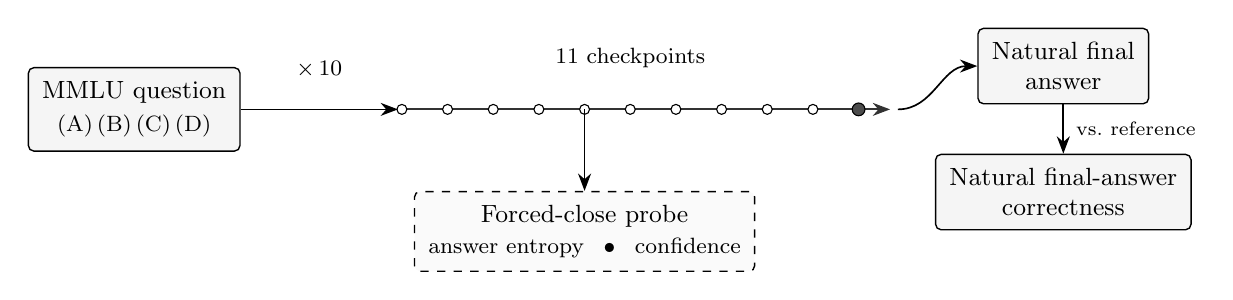
\begin{tikzpicture}[
  font=\small,
  >={Stealth[length=2.2mm]},
  box/.style={
    draw,
    rounded corners=2pt,
    align=center,
    inner sep=5pt,
    line width=0.5pt
  },
  qbox/.style={box, fill=black!4},
  resbox/.style={box, fill=black!4},
  probebox/.style={box, dashed, fill=black!2},
  cp/.style={
    circle,
    draw,
    fill=white,
    inner sep=0pt,
    minimum size=3.6pt,
    line width=0.4pt
  },
  cpend/.style={
    circle,
    draw,
    fill=black!70,
    inner sep=0pt,
    minimum size=4.6pt,
    line width=0.4pt
  },
  traj/.style={line width=0.7pt, black!80},
  arr/.style={
    -{Stealth[length=2.2mm]},
    line width=0.6pt
  }
]

\def\xL{3.4}
\def\xR{9.2}
\pgfmathsetmacro\xM{(\xL+\xR)/2}

% MMLU question
\node[qbox] (q) at (0,0)
  {MMLU question\\[1pt]
   \footnotesize (A)\,(B)\,(C)\,(D)};

% Natural reasoning trajectory
\draw[traj,->] (\xL,0) -- (\xR+0.4,0);

\foreach \i in {0,...,10}{
  \pgfmathsetmacro\cx{\xL + (\xR-\xL)*\i/10}
  \ifnum\i=10
    \node[cpend] at (\cx,0) {};
  \else
    \node[cp] at (\cx,0) {};
  \fi
}

\draw[arr] (q.east) -- (\xL-0.05,0);

\node[font=\footnotesize] at (2.35,0.5)
  {$\times\,10$};

\node[font=\footnotesize] at (\xM,0.65)
  {11 checkpoints};

% Natural final answer and correctness
\node[resbox] (nfa) at (11.8,0.55)
  {Natural final\\answer};

\node[resbox] (corr) at (11.8,-1.05)
  {Natural final-answer\\correctness};

\draw[arr] (\xR+0.5,0)
  to[out=0,in=180] (nfa.west);

\draw[arr] (nfa.south) --
  node[right=1pt, font=\scriptsize] {vs.\ reference}
  (corr.north);

% Representative forced-close probe
\pgfmathsetmacro\cxp{\xL + (\xR-\xL)*0.4}

\node[probebox] (probe) at (\cxp,-1.55)
  {Forced-close probe\\
   \footnotesize answer entropy \enspace $\bullet$ \enspace confidence};

\draw[arr] (\cxp,0) -- (probe.north);

\end{tikzpicture}

\caption{
Overview of the experimental pipeline. Each MMLU question produces ten
natural reasoning trajectories, with forced-close probes applied at eleven
points along each trajectory.
}
\label{fig:pipeline}

\end{figure*}

\subsection{Checkpoint Probing}
\label{sec:checkpoint-probing}

To compare intermediate stages across trajectories of different lengths, we divided each reasoning trajectory into 10\% increments, yielding eleven checkpoints from 0\% to 100\%. At each checkpoint, only the reasoning generated up to that point was retained.

For each checkpoint, we used the original question and answer choices together with the corresponding partial reasoning chain. We then prematurely terminated the reasoning and forced the model to produce an answer using constrained deterministic decoding. We refer to the resulting response as the \emph{checkpoint answer}. Each probe was conducted independently of the original generation, so that the natural trajectory and its original final answer were retained. The checkpoint answers therefore provide measurements of the model's answer at different stages of reasoning without altering the natural generation.


\subsection{Extracting Uncertainty and Confidence Signals}
\label{sec:signal-extraction}

We extracted complementary measurements from both the uninterrupted reasoning trajectories and the checkpoint probes. Reasoning-token entropy was computed from the model's predictive distribution at each token along the natural reasoning trajectory. At each checkpoint, the logits corresponding to the four answer choices were normalized to obtain a probability distribution over A--D, from which answer-choice entropy was calculated. Verbalized confidence was recorded both at the end of the model's uninterrupted natural response and from each forced checkpoint response.


\subsection{Statistical Analysis}
\label{sec:analysis}

Our analyses used the correctness of the natural final answer as the outcome and were restricted to trajectories with a valid parsed A--D answer. Confidence intervals were estimated from 5,000 bootstrap samples drawn by resampling questions within each subject, while keeping all trajectories generated from the same question together.

For the within-question analysis, we considered only questions that produced at least one correct and one incorrect evaluable trajectory. Signal values were averaged separately across correct and incorrect trajectories within each question, and the resulting question-level differences were then averaged with equal weight across questions. Calibration results were evaluated using ECE and reliability diagrams.


\section{Results}
\label{sec:results}

\subsection{Overall Accuracy and Response Evaluability}

Of the 5{,}000 generated trajectories, 3{,}550 (71.0\%) yielded an evaluable natural A--D answer, with evaluability varying substantially across subjects (Table~\ref{tab:cohort}). Unevaluable responses either reached the generation limit without producing a final answer or produced an output that could not be parsed as one of the four candidate choices. Among evaluable trajectories, natural final-answer accuracy was 89.4\%. Only 84 of the 500 questions produced both correct and incorrect evaluable trajectories, providing the set of questions used for the within-question comparison.


\begin{table*}[t]
\centering
\begin{tabular}{lrrrr}
\toprule
Subject & Evaluable, $n$ (\%) & Correct / Incorrect & Accuracy (\%) & Mixed-outcome questions \\
\midrule
Mathematics & 598 (59.8) & 588 / 10 & 98.3 & 6 \\
Physics & 647 (64.7) & 549 / 98 & 84.9 & 21 \\
Chemistry & 578 (57.8) & 503 / 75 & 87.0 & 21 \\
Biology & 847 (84.7) & 747 / 100 & 88.2 & 18 \\
Psychology & 880 (88.0) & 785 / 95 & 89.2 & 18 \\
\midrule
\textbf{Total} & \textbf{3{,}550 (71.0)} & \textbf{3{,}172 / 378} & \textbf{89.4} & \textbf{84} \\
\bottomrule
\end{tabular}

\caption{Natural-answer evaluability and accuracy by subject. Each subject contributed 1{,}000 trajectories from 100 questions with ten trajectories per question. Accuracy is calculated among evaluable trajectories. Mixed-outcome questions contain at least one correct and one incorrect evaluable trajectory.}
\label{tab:cohort}
\end{table*}


\subsection{Uncertainty and Confidence Across Reasoning}
\label{sec:results-rq1}

Figure~\ref{fig:signal_evolution} shows the mean uncertainty and confidence measures across stages of reasoning. Reasoning-token entropy rises sharply over approximately the first 20--30\% of reasoning before remaining relatively stable for the rest of the trajectory. Answer-choice entropy remains high early in reasoning and declines steadily over the latter portion of the trajectory. In contrast, verbalized confidence remains consistently high, increasing only modestly from about 90\% to 94\%.

A closer look at the answer-choice entropy profiles in Figure~\ref{fig:answer_entropy_outcome} shows that this overall decline follows a similar pattern for both correct and incorrect final outcomes. Across all evaluable trajectories, shown by the solid lines, answer-choice entropy declines substantially for both groups. Trajectories yielding incorrect answers have higher answer-choice entropy through much of reasoning, but both groups approach low entropy near the endpoint. The dashed lines show that the same overall pattern remains when the analysis is restricted to the 84 mixed-outcome questions. Moreover, the correct and incorrect profiles are also substantially closer than in the full evaluable set.

\begin{figure}[t]
\centering
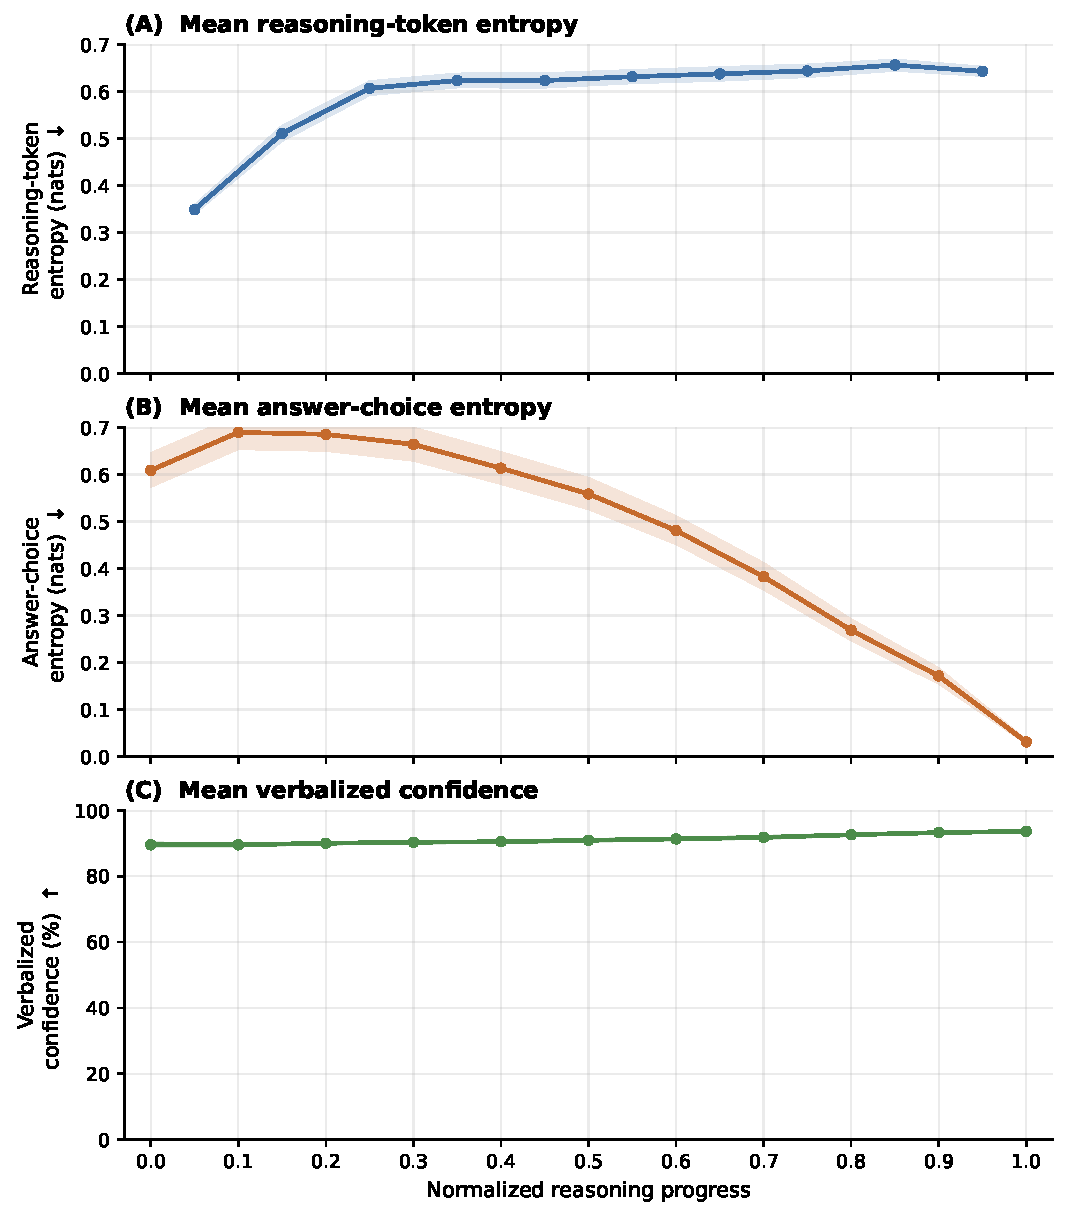
\includegraphics[width=\linewidth]{fig1_signal_evolution}
\caption{Mean reasoning-token entropy, answer-choice entropy, and verbalized confidence across reasoning progress. Values are shown at the eleven normalized reasoning positions from 0\% to 100\% in 10\% increments. Reasoning-token entropy is derived from the natural reasoning trajectory, while answer-choice entropy and verbalized confidence are obtained from checkpoint probes. Arrows accompanying the y-axis labels indicate the direction corresponding to greater certainty or confidence. Shaded bands show bootstrapped 95\% confidence intervals.}
\label{fig:signal_evolution}
\end{figure}

\begin{figure*}[t]
\centering
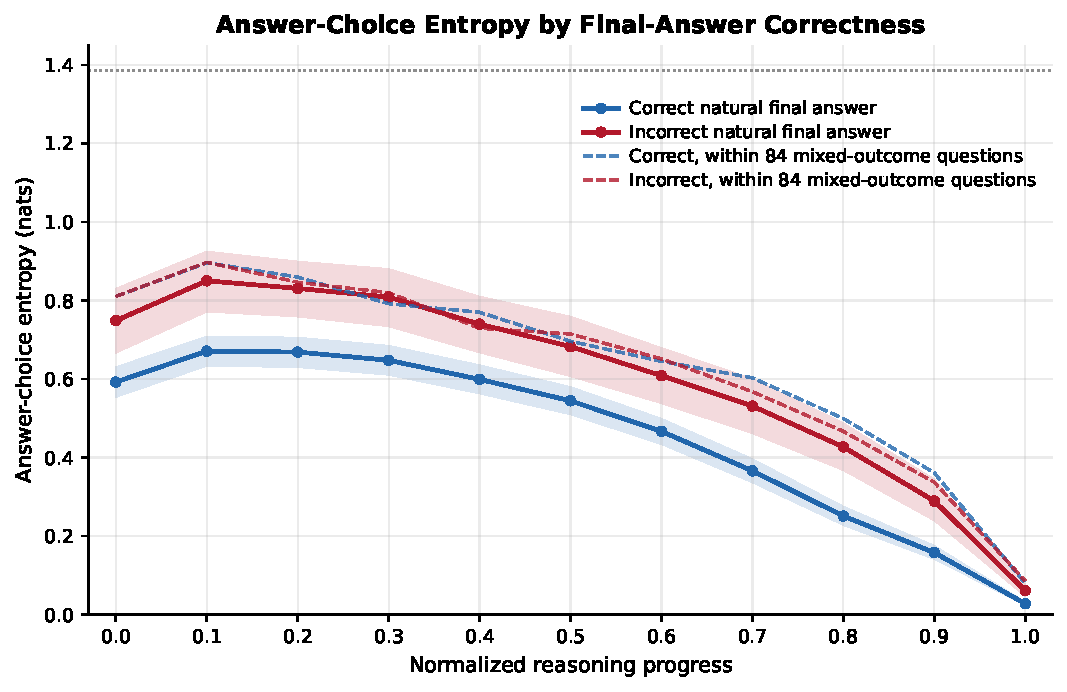
\includegraphics[width=0.78\textwidth]{fig5_answer_entropy_by_outcome}
\caption{Answer-choice entropy across reasoning progress by natural final-answer correctness. Solid lines show mean profiles across all evaluable trajectories, while dashed lines restrict the comparison to the 84 questions that produced both correct and incorrect evaluable trajectories.}
\label{fig:answer_entropy_outcome}
\end{figure*}

\subsection{Within-Question Differences}
\label{sec:results-rq2}

Figure~\ref{fig:within_question} compares the relationship between reasoning-token entropy and correctness in two settings. Panel A shows all evaluable trajectories, where responses yielding incorrect final answers have higher reasoning-token entropy than those yielding correct final answers, with a mean difference of approximately 0.13~nats. Panel B restricts the comparison to the 84 questions that produced both correct and incorrect evaluable trajectories. Within these questions, the mean incorrect-minus-correct difference is only +0.0113~nats (95\% CI [0.0002, 0.0225]). As shown by the individual question estimates in Panel B, this difference is not consistent across questions. Some questions have higher mean entropy among trajectories yielding incorrect answers, while others have higher mean entropy among trajectories yielding correct answers.

\begin{figure*}[t]
\centering
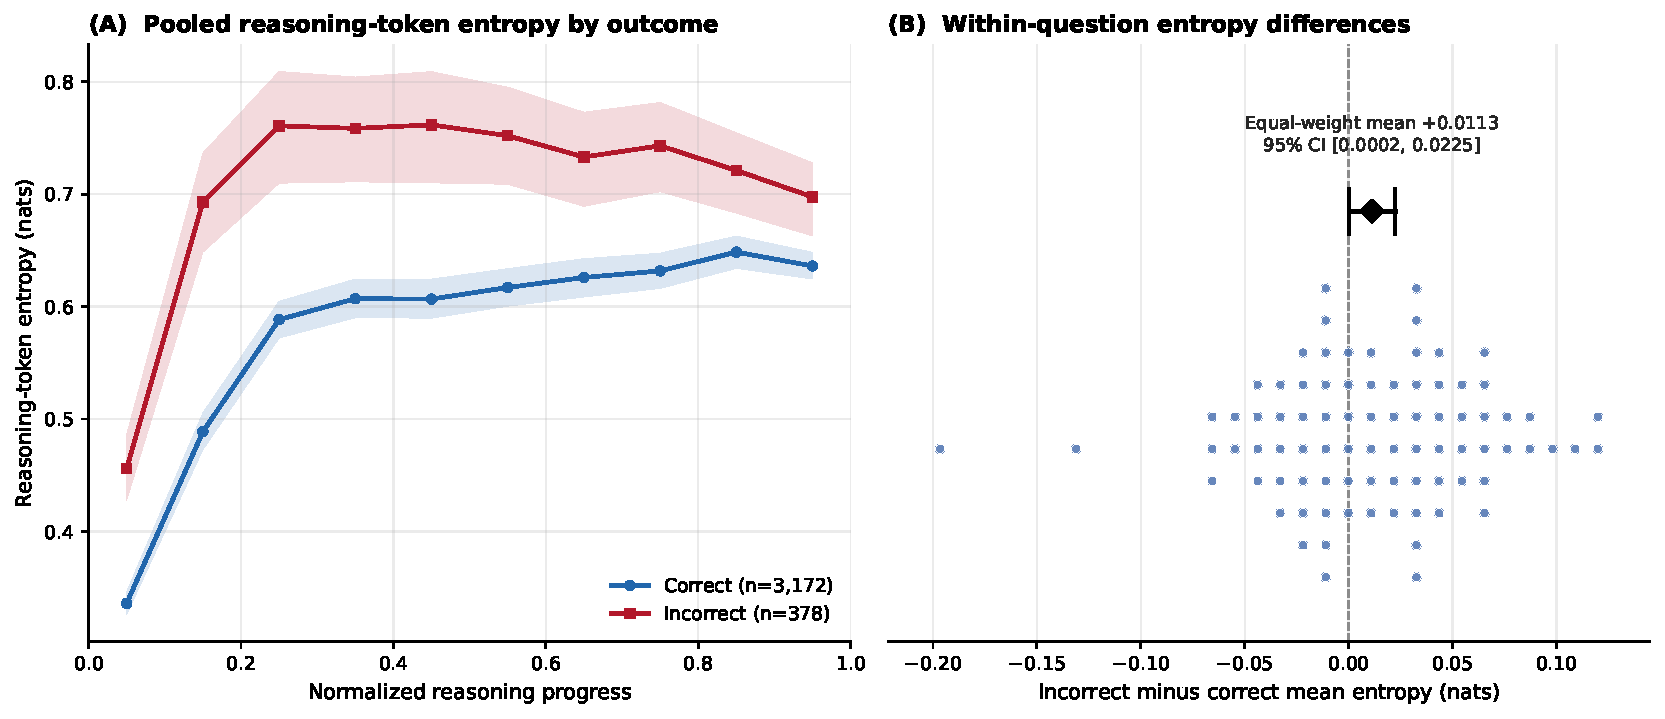
\includegraphics[width=\textwidth]{fig3_within_question}
\caption{Reasoning-token entropy by natural final-answer correctness. Panel A shows mean entropy across normalized reasoning progress for evaluable trajectories ending in correct and incorrect answers. Panel B compares these outcomes within the 84 questions for which both were observed. Each point shows, for one question, the difference between mean entropy across its incorrect and correct trajectories (incorrect minus correct); positive values therefore indicate higher entropy for incorrect trajectories. The black diamond and error bar show the equal-weight mean difference across questions and its 95\% confidence interval, and the dashed line marks zero difference.}
\label{fig:within_question}
\end{figure*}


\subsection{Comparing Reliability Signals}
\label{sec}

The uncertainty and confidence measures also vary in their ability to discriminate as reasoning progresses. Figure~\ref{fig:discrimination} shows their discrimination across the eleven normalized reasoning positions. Reasoning-token entropy provides its strongest discrimination at approximately 20--30\% of the trajectory, with an AUROC near 0.77, before gradually declining toward the endpoint. Answer-choice entropy provides more modest discrimination early in reasoning before improving later in the trajectory. Verbalized confidence is close to chance early and also becomes more discriminative toward the endpoint.

\begin{figure*}[t]
\centering
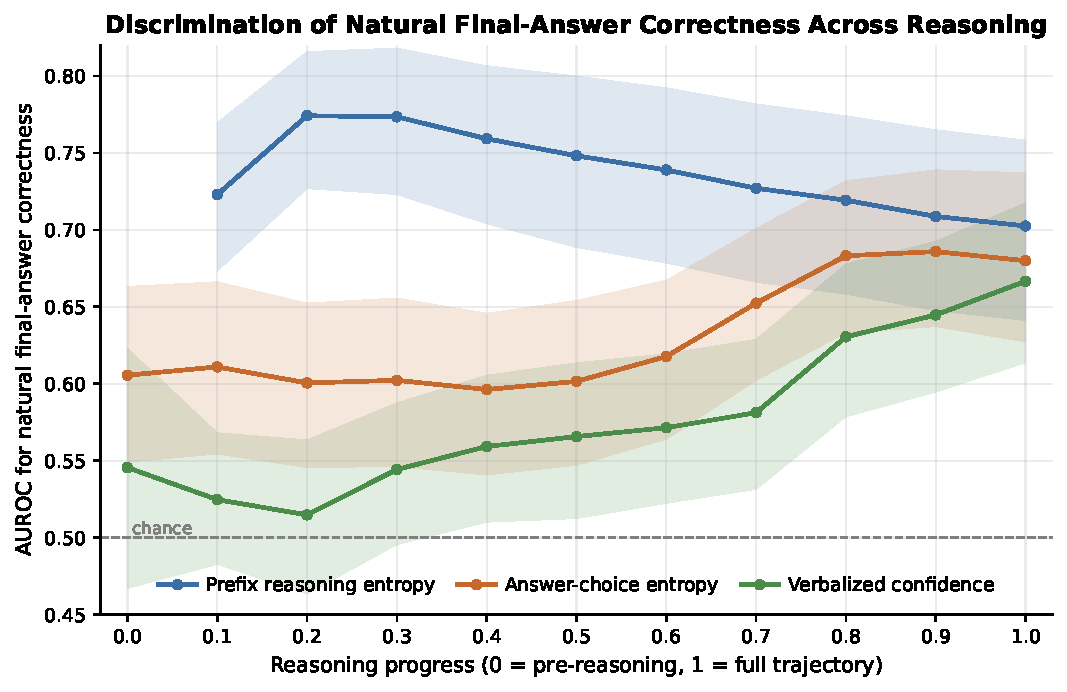
\includegraphics[width=0.78\textwidth]{fig2_discrimination}
\caption{Discrimination of natural final-answer correctness across reasoning progress. Shaded bands show bootstrapped 95\% confidence intervals.}
\label{fig:discrimination}
\end{figure*}

At the endpoint, both selected-answer probability and verbalized confidence are overconfident relative to the observed accuracy of 0.894. Mean selected-answer probability is 0.994 with an ECE of 0.100, while mean verbalized confidence is 0.936 with an ECE of 0.044.



\section{Discussion}
\label{sec:discussion}

\subsection{Uncertainty and Confidence Evolve Differently During Reasoning}

The three signals follow clearly different patterns as reasoning progresses. Answer-choice entropy falls through much of the trajectory, meaning that the model's probability distribution becomes increasingly concentrated on one answer relative to the alternatives. Figure~\ref{fig:answer_entropy_outcome} shows that this increasing concentration occurs for trajectories that ultimately answer both correctly and incorrectly. The model can therefore become increasingly certain of a particular answer even when that answer is wrong. \citet{xu2026entropy} report a related result, finding that reasoning can converge toward both correct and incorrect answers. Together, these findings show that increasing certainty about an answer does not necessarily indicate that the eventual answer will be correct.

Verbalized confidence shows a different pattern. It remains consistently high even while the model's answer distribution changes substantially over the course of reasoning. Reported confidence therefore does not closely track the changes in predictive uncertainty captured by answer-choice entropy. This is consistent with \citet{ulmer2026anthropomimetic}, who argue that verbalized uncertainty is shaped by how models are trained and prompted to communicate uncertainty rather than providing direct access to an underlying uncertainty state. The different temporal patterns in Figure~\ref{fig:signal_evolution} therefore reflect more than differences in numerical scale.

\subsection{Uncertainty Differences Between Outcomes Weaken Within Questions}

Panel A of Figure~\ref{fig:within_question} shows a clear separation across all evaluable trajectories, with substantially higher reasoning-token entropy for trajectories that ultimately answer incorrectly. This relationship becomes much weaker when the underlying question is held fixed. In Panel B, the average difference between the two outcomes is small, and individual questions show differences in both directions. The same tendency is visible for answer-choice entropy in Figure~\ref{fig:answer_entropy_outcome}. The profiles for the two outcome groups are more clearly separated across all evaluable trajectories than when the comparison is restricted to the 84 questions that produce both outcomes.

Taken together, these results suggest that some of the correct--incorrect separation observed across the benchmark comes from differences between questions rather than from a consistent difference between successful and unsuccessful attempts at the same problem. One possible explanation is question difficulty. Questions that are harder for the model may both produce higher uncertainty and be answered incorrectly more often. Pooling these questions with easier ones would then strengthen the apparent relationship between uncertainty and correctness even if the signal provides much less separation among different attempts at the same question. In this setting, an uncertainty measure may reflect which questions the model tends to struggle with more strongly than it reflects which sampled attempt at a particular question will succeed. \citet{taubenfeld2025confidence} report a related distinction, showing that confidence measures evaluated across questions need not be equally effective at distinguishing correct and incorrect sampled responses to the same question.

\subsection{Reliability Signals Are Informative at Different Stages}

The three signals have substantially different discrimination early in reasoning but become much more similar near the endpoint in Figure~\ref{fig:discrimination}. Their similar endpoint discrimination therefore hides an important difference in when they become informative. Reasoning-token entropy is particularly notable because its discrimination is strongest around the same 20--30\% point at which its mean changes most rapidly in Figure~\ref{fig:signal_evolution}. This temporal alignment does not show that one pattern causes the other, but it indicates that reasoning-token entropy has its strongest relationship with final-answer correctness relatively early rather than building toward the final answer.

The average value of a signal and its discrimination can also change independently. Verbalized confidence changes little in magnitude even though its discrimination improves toward the endpoint. Answer-choice entropy provides a complementary example. Its average value falls for both outcome groups while its discrimination improves later in reasoning. Both cases show why the temporal shape of a signal should not be interpreted as a direct measure of how informative that signal is about correctness.

Verbalized confidence provides a further example of why the way a reliability signal is evaluated matters. At the endpoint, its ECE is 0.044, compared with 0.100 for selected-answer probability, making verbalized confidence appear better calibrated by this measure. Its relatively low calibration error may partly reflect the close match between the model's high overall accuracy and its consistently high reported confidence. A confidence signal can therefore be well calibrated in this aggregate sense without closely distinguishing which individual responses are likely to be wrong.

This distinction is important because verbalized confidence is especially easy to obtain from a language model. A user can simply ask how confident the model is in its answer. Prior work has shown that directly elicited confidence can be well calibrated \citep{tian2023calibration}, while \citet{taubenfeld2025confidence} found that their most calibrated confidence measure was the least effective under their within-question evaluation. Our results add a temporal perspective to this distinction. Verbalized confidence remains consistently high even as the model's predictive uncertainty changes substantially during reasoning. The usefulness of verbalized confidence therefore depends both on what it is being used to assess and when it is measured.

\subsection{Future Work}

The first priority is to determine whether these findings generalize across larger reasoning models and different model families. Studying several models on the same questions would also make it possible to model question difficulty more directly. In particular, item-response models could separate variation associated with item difficulty from differences in model capability. This would allow future work to test whether reasoning-token entropy remains associated with correctness after question difficulty is taken into account, providing a more direct test of the explanation suggested by the within-question results.

A second direction is to extend the analysis beyond multiple-choice questions. The fixed A--D answer space makes answer-choice entropy straightforward to measure, but it remains unclear whether open-ended responses would show the same increase in certainty for both correct and incorrect outcomes. Open-generation settings would require a different answer-level uncertainty measure. Semantic entropy, for example, could characterize uncertainty over semantically distinct responses rather than exact generated strings \citep{kuhn2023semantic,farquhar2024semantic}. This would make it possible to test whether increasing answer certainty can likewise occur for incorrect outcomes beyond the multiple-choice setting.



\section{Literature Review}

\subsection{Reasoning Models and Explicit Reasoning}

The role of explicit reasoning in language models has expanded substantially since the introduction of chain-of-thought prompting. \citet{wei2022chain} showed that eliciting intermediate reasoning steps could improve performance on a range of reasoning tasks, while \citet{wang2023selfconsistency} demonstrated that the same problem can produce distinct sampled reasoning paths whose final answers can be aggregated through self-consistency. More recent work has placed greater emphasis on the computation performed during inference itself. \citet{snell2025scaling} showed that additional test-time computation can improve reasoning when allocated effectively, with the appropriate strategy depending on problem difficulty. Reasoning models such as DeepSeek-R1 further extend this setting by generating longer reasoning processes that can include behaviours such as reflection, verification, and strategy adjustment \citep{guo2025deepseek}. As explicit reasoning has become longer and more variable, the trajectory itself has increasingly become an object that can be analyzed rather than only a mechanism for producing a final answer.

\subsection{Uncertainty at the Response Level}

A major line of uncertainty research characterizes reliability using information from the model's predictive distribution. For autoregressive models, this information can be summarized at different levels of a generated response. \citet{malinin2021uncertainty} developed a probabilistic framework for uncertainty estimation in autoregressive structured prediction that considers uncertainty at both individual token positions and over complete generated sequences. Probability-based measures have since remained one of several established approaches to confidence estimation in large language models \citep{geng2024survey}. Their use in natural language generation is complicated, however, by the many ways in which similar content can be expressed. Low probability may reflect variation in wording or syntax without necessarily indicating uncertainty about the substance of an answer. This limitation has motivated methods that estimate uncertainty from variation across several possible responses rather than from the probability of a single output.

Repeated generation provides another source of reliability information by exposing variation in the responses a model can produce for the same input. The variability revealed by methods such as self-consistency can therefore also provide evidence about how concentrated the model's possible answers are \citep{wang2023selfconsistency}. For open-ended generation, however, disagreement between strings can overstate meaningful uncertainty when different responses express the same answer. \citet{kuhn2023semantic} address this problem through semantic uncertainty, which groups sampled generations according to their meaning and estimates uncertainty over these semantic alternatives. \citet{farquhar2024semantic} subsequently apply semantic entropy to confabulation detection, showing that uncertainty over meaning can identify unreliable generations across models and question-answering settings. This line of work therefore shifts attention from the probability of one particular realization toward the distribution of semantically distinct responses that a model may produce.

\subsection{Confidence and Complementary Reliability Signals}

Rather than inferring uncertainty from probabilities or variation across generations, another line of work asks whether language models can assess the reliability of their own answers. \citet{kadavath2022know} found that larger language models could provide informative self-evaluations of whether their responses were correct, with this ability generally improving with scale and with access to additional sampled responses. \citet{tian2023calibration} extended this direction to models fine-tuned with human feedback and showed that directly elicited confidence could be better calibrated than confidence derived from conditional probabilities. The quality of these reports is nevertheless sensitive to how they are obtained. \citet{yang2026verbalized} find substantial variation across models, datasets, and elicitation strategies, while \citet{ulmer2026anthropomimetic} argue that verbalized uncertainty should be understood as linguistic behaviour shaped by how models are trained and prompted to communicate uncertainty. Verbalized confidence can therefore provide useful information about answer reliability without necessarily providing direct access to an underlying uncertainty state.

More broadly, reliability signals need not preserve the same relationship with correctness across models or evaluation settings. \citet{flores2026confidence} show that supervised fine-tuning can substantially alter the relationship between several confidence measures and output quality. \citet{kumaran2026reported} similarly finds that verbal and probability-based confidence can relate differently to objective correctness and subsequent model behaviour. \citet{taubenfeld2025confidence} show that standard calibration and between-question confidence measures can be poor predictors of whether a confidence signal distinguishes correct from incorrect sampled responses to the same question. Their results demonstrate that a signal can characterize differences among questions while providing substantially less information for selecting among responses to a fixed problem. Taken together, this work suggests that the usefulness of a reliability signal depends both on what information it captures and on the comparison used to evaluate it. Most of these approaches nevertheless characterize completed responses or sets of completed responses, while explicit reasoning makes it possible to examine how reliability-related signals develop as reasoning unfolds.

\subsection{Reliability During Reasoning}

Recent work has begun to treat uncertainty and confidence as temporally structured quantities rather than reducing an entire reasoning process to a single score. \citet{mao2025temporalizing} analyze confidence throughout chain-of-thought as a temporal signal and show that its evolution contains information related to reasoning success. Entropy-based studies reach a similar broader conclusion through different measurements. Local increases, rebounds, and other irregularities in token entropy have been associated with reasoning failures \citep{zhu2026edis}, while the shape of answer-uncertainty trajectories can be more informative than the total change in uncertainty alone \citep{zhao2026entropytrajectory}. Other work characterizes uncertainty profiles through properties such as their slope and linearity, finding that differences between successful and unsuccessful reasoning can emerge relatively early in generation \citep{grunefeld2026tracing}. Using uncertainty measured from intermediate answer completions, \citet{xu2026entropy} identify a transition from a region of higher uncertainty toward a more stable confidence region. These studies differ in both the quantities they measure and the temporal patterns they report. Their common implication is therefore not a single characteristic shape of reasoning uncertainty, but that its temporal organization can contain information that is lost when the reasoning process is summarized by an endpoint or global scalar.

Related work has examined intermediate reasoning more directly by probing partial trajectories before their natural completion. \citet{ballon2026probing} truncate reasoning traces at different depths and use the resulting prefixes to probe the model's distribution over candidate answers, finding that additional relevant reasoning contributes answer information beyond effects attributable to context length or generic reasoning style. Using a related forced-completion procedure, \citet{datta2026decide} find that elicited answers often become stable substantially before the complete reasoning trace has been generated. \citet{zhou2025landscape} take a different approach by representing successive reasoning states according to their relationships with candidate answers and identifying distinct trajectory structures associated with different outcomes. Together, these approaches show that partial reasoning traces can already contain substantial answer-relevant information and that observable answer behaviour can evolve well before generation is complete. At the same time, conclusions drawn from such interventions concern behaviour elicited from partial traces and should not automatically be interpreted as direct observations of an internal decision state.

Several of these process-level studies also compare uncertainty profiles or trajectory properties across correct and incorrect outcomes \citep{zhu2026edis,zhao2026entropytrajectory,grunefeld2026tracing,zhou2025landscape}. Recent work therefore already establishes that uncertainty can evolve systematically during reasoning, that partial trajectories can contain answer-relevant information, and that characteristics of reasoning trajectories can be associated with eventual correctness. Separately, work on repeated completed responses shows that relationships observed across questions need not be preserved when correct and incorrect samples are compared within the same underlying problem \citep{taubenfeld2025confidence}. These lines of research leave a less developed intersection between multi-signal reliability analysis and process-level reasoning analysis. In particular, comparatively less is known about how complementary predictive and verbalized reliability signals relate as they evolve through the same reasoning trajectories, and how their relationship with correctness changes when the underlying question is held fixed.




\section{Conclusions}
\label{sec:conclusions}

Taken together, our findings show that reliability during reasoning cannot be understood from a single uncertainty or confidence signal. The results show that these signals capture different aspects of model behaviour and become informative at different stages of reasoning. In particular, the model can become increasingly certain of an answer even when that answer is ultimately incorrect, while verbalized confidence remains consistently high despite substantial changes in its predictive uncertainty. We also find that the relationship between reasoning-token entropy and correctness becomes much weaker when the underlying question is held fixed, suggesting that benchmark-wide relationships can partly reflect differences between questions. Together, these findings show that reliability cannot be characterized by a single signal or endpoint measurement alone. Understanding what a reliability signal reveals requires considering both how it evolves during reasoning and the level at which its relationship with correctness is evaluated.


\section{Limitations}
\label{sec:limitations}

This study is limited to SmolLM3-3B and five high-school subjects from MMLU. The question sample is also limited to 100 questions per subject, with ten stochastic trajectories generated for each question, so the observed trajectories represent only a sample of the reasoning paths the model could produce. The conclusions therefore apply to a relatively small reasoning model in a multiple-choice setting and may not extend to other models, tasks, or forms of generation. The analyses are also based only on trajectories with an evaluable natural answer. Of the 5,000 generated trajectories, 3,550 met this criterion, and evaluability varied substantially across subjects. Because trajectories without an evaluable natural answer are excluded from correctness-based analyses, the analyzed cohort may not represent the full distribution of model behaviour. The within-question analysis was further restricted to 84 questions that produced both correct and incorrect evaluable trajectories, limiting how broadly these comparisons can be interpreted.

%The measured signals also have important interpretive limits. Reasoning-token entropy reflects uncertainty in next-token prediction and should not be interpreted as a direct measure of whether the reasoning itself is correct. Similarly, answer-choice entropy measures how concentrated the model's probability is over the available answer choices, so decreasing entropy can reflect increasing certainty even when the selected answer is wrong. The checkpoint probes provide a way to measure answer-level uncertainty and verbalized confidence at intermediate stages, but they require prematurely terminating the reasoning and eliciting an answer that the model would not otherwise have produced at that point. These measurements therefore characterize the model's state under the probing procedure rather than an unobserved natural intermediate answer. Verbalized confidence is also prompt-dependent and may reflect how the model communicates uncertainty rather than its predictive uncertainty directly.


\bibliography{references}

\end{document}
